\chapter{Problema de investigación}
\label{Problemática}

\section{Situación Problemática}

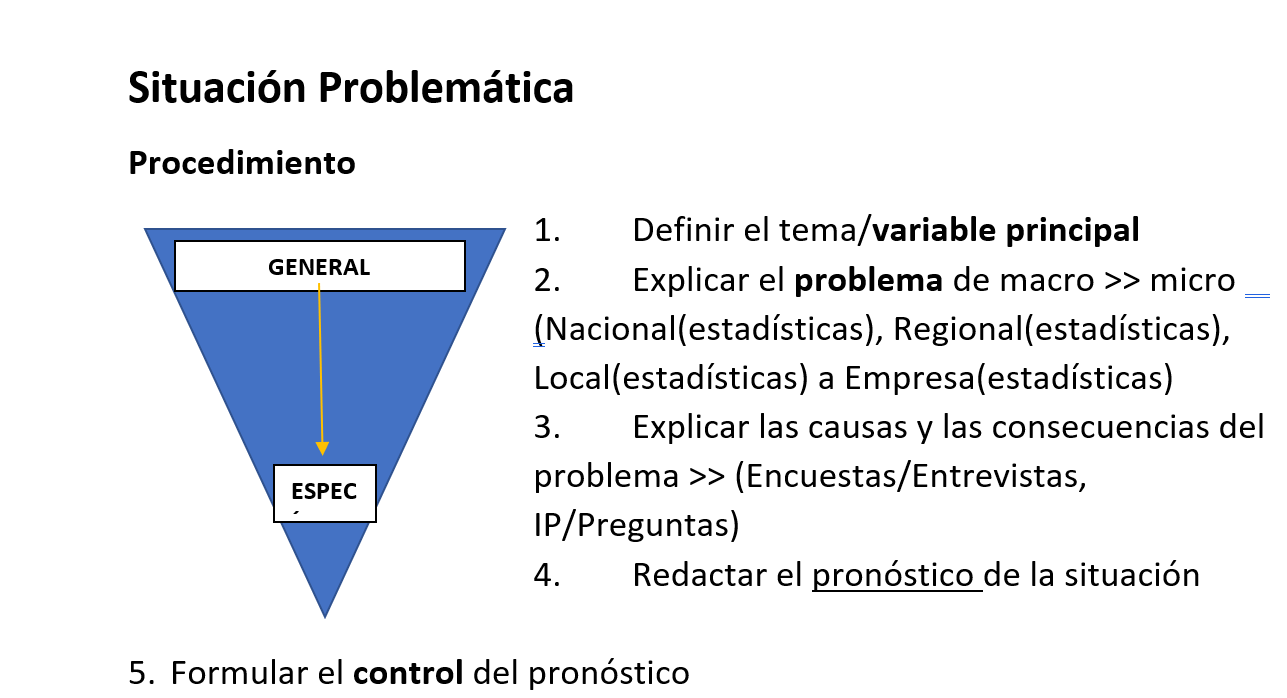
\includegraphics[scale=0.5]{img/problem_sec.png}

\section{Pregunta de Investigación}

La formulación de un problema consiste en la presentación oracional del mismo, es decir, “reducción del problema a términos concretos, explícitos, claros y precisos” (Tamayo, 1993), y es “la concreción del planteamiento en una pregunta precisa y delimitada en cuanto a espacio, tiempo y población (si fuere el caso)”. (Fidias G. Arias, 2006)

Debe cumplir:
\begin{itemize}
    \item Carecer de expresiones que implican juicios de valor: bueno, malo, mejor, etc.
    \item No originar respuestas tales como SI o No
    \item Estar delimitados en cuanto a tiempo y espacio y población
\end{itemize}

Puede ser de forma \textbf{Interrogativa/afirmativa}.


Por ejemplo:

Ejemplo 1:¿Cuál es el impacto de la satisfacción en la lealtad de los clientes en los restaurantes de comida china en Lima Metropolitana, 2019?

Ejemplo 2: ¿Cómo la alta rotación del personal incide en la productividad de la empresa Muebles Finos S.A.C. de la ciudad de Arequipa, 2019?

Ejemplo 3: ¿Cuáles son los factores que inciden en la motivación del personal de ventas de la empresa Jugos del Norte S.A. durante el periodo de 2018 y 2019?

\textbf{Elementos:}

\textbf{La interrogante:} es la pregunta clave que se planteará.

\textbf{Variable o variables:} la variable o variables que forman parte del estudio. En el caso de un estudio descriptivo será una variable, mientras que en un estudio correlacional serán dos variables.

\textbf{Enlace o relacionante:} el vínculo con el cual se relaciona las variables.

\textbf{Población:} es generalmente la colección de individuos u objetos que son el foco principal de la investigación científica, y que serán observados, encuestados o medidos.

\textbf{Delimitación espacial:} el lugar o zona geográfica que comprende el estudio. También comprende el ámbito específico de estudio, como por ejemplo puede ser una empresa determinada o conjunto de negocios (como los cinemas).

\textbf{Delimitación temporal:} el período de tiempo que comprende el estudio.



